% !Mode:: "TeX:UTF-8"
\documentclass{tufte-handout}

\title{Git hands-on, part I: single user operations}

\author{S\'ebastien Dawans}

\date{21 January 2014} % without \date command, current date is supplied

%\geometry{showframe} % display margins for debugging page layout
\usepackage[utf8]{inputenc}
\usepackage{graphicx} % allow embedded images
  \setkeys{Gin}{width=\linewidth,totalheight=\textheight,keepaspectratio}
  \graphicspath{{graphics/}} % set of paths to search for images
\usepackage{amsmath}  % extended mathematics
\usepackage{booktabs} % book-quality tables
\usepackage{units}    % non-stacked fractions and better unit spacing
\usepackage{multicol} % multiple column layout facilities
\usepackage{lipsum}   % filler text
\usepackage{fancyvrb} % extended verbatim environments
  \fvset{fontsize=\normalsize}% default font size for fancy-verbatim environments
\usepackage{listings}
\lstset{showstringspaces=false}
\usepackage[usenames]{xcolor}

\lstdefinestyle{BashInputStyle}{
  language=bash,
  basicstyle=\footnotesize\ttfamily,
  %numbers=left,
  %numberstyle=\tiny,
  %numbersep=3pt,
  frame=tb,
  columns=fullflexible,
  backgroundcolor=\color{yellow!20},
  linewidth=0.95\linewidth,
  xleftmargin=0.05\linewidth,
  moredelim=**[is][\color{red}]{§}{§},
  moredelim=**[is][\color{OliveGreen}]{`}{`}
}

% Standardize command font styles and environments
\newcommand{\doccmd}[1]{\texttt{\textbackslash#1}}% command name -- adds backslash automatically
\newcommand{\docopt}[1]{\ensuremath{\langle}\textrm{\textit{#1}}\ensuremath{\rangle}}% optional command argument
\newcommand{\docarg}[1]{\textrm{\textit{#1}}}% (required) command argument
\newcommand{\docenv}[1]{\textsf{#1}}% environment name
\newcommand{\docpkg}[1]{\texttt{#1}}% package name
\newcommand{\doccls}[1]{\texttt{#1}}% document class name
\newcommand{\docclsopt}[1]{\texttt{#1}}% document class option name
\newenvironment{docspec}{\begin{quote}\noindent}{\end{quote}}% command specification environment

\begin{document}

\maketitle% this prints the handout title, author, and date

\begin{abstract}
\noindent
This handout is a walkthrough for a 2-hour hands-on session on the Git.
The goal is to offer a first experience with Git on the client side using Git's native command-line interface to learn basic concepts about Source Code Management with Git.
The intended audience for this session is one or more developers having already received in introduction to basic Git concepts, such as those available in the presentations folder of the git-slides repository \url{https://github.com/sdawans/git-slides}.
This session deals exclusively with single-user repositories, ideal for training multiple people at the same time without having to deal with multi-developer workflows at the very beginning.
\end{abstract}

%\printclassoptions

\section{Introduction}\label{sec:intro}

Git is a Source Code Management (SCM) system with three key design principles.
Git is \textbf{Distributed}, \textbf{Fast} and \textbf{Reliable}.
It is very different from not only centralized SCMs like SVN, but also other forms of distributed SCMs like Mercurial.
To follow this introductory session, it's best to clear your mind of everything you know about other SCMs, as some false similarities are often misleading.

\section{Preparation}

In preparation of this course, each participant must have a properly installed and configured command-line client for Git, and access to the git repositories hosted on a local instance of Gitlab.

\subsection{Installing a Git client}\label{sec:preparation}

Linux and MacOS X users will find the native git client in their respective package managers.
Windows users should install the latest versions of TortoiseGit \marginnote{\url{http://code.google.com/p/tortoisegit/}} (for the TortoisePlink.exe binary) and msysgit \marginnote{\url{http://code.google.com/p/msysgit/}}, in that order.
In the msysgit installation wizard, the path to TortoisePlink.exe should be selected when prompted for the SSH connexion handler.
Furthermore, windows users will need puttygen.exe and pageant.exe, available on the Putty website \marginnote{\url{http://www.putty.org/}}.

An SSH keypair must be generated puttygen.
The contents of the public key should be copy/pasted in your Gitlab user settings while the private key should be stored locally and added to pageant.
You may write a batch script to automatically run pageant at system boot and load the private key.

\subsection{Configuring Git}

People are an important aspect in any SCM, as every code change must be attributed to a certain author.
\marginnote{In fact, Git manages users thoroughly by seperating \textbf{authors} from \textbf{committers}.
An author is the person who (originally) writes a certain patch (new code, code modification), while the committer is the person who applies the said changes on a particular code base.}
The user must thus identify himself before using a git client.
Git uses a global \texttt{user.name} and \texttt{user.email} setting applied to all projects, which is overridable locally for a specific project.
For this session, we will set the global settings for all the projects on the machine:

\begin{lstlisting}[style=BashInputStyle]
  $ git config --global user.name "First Last"
  $ git config --global user.email "first.last@example.com"
\end{lstlisting}

Another useful configuration (already default on msysgit) is to enable color output in the console.

\noindent To do so:

\begin{lstlisting}[style=BashInputStyle]
  $ git config --global color.ui true
\end{lstlisting}

Windows users who are not comfortable with Vim, the default commit-message editor in msysgit, can define a \texttt{core.editor} option to another editor.
For example, to use Notepad++ as default:

\marginnote{According to \url{http://starikovs.com/2012/11/06/git-core-editor-windows/}, you can simple write 'notepad++' instead of the full path to the application if it is correctly defined in your PATH environment variable.}
\begin{lstlisting}[style=BashInputStyle]
  $ git config --global core.editor
    "'C:/path/to/notepad++.exe' -multiInst -notabbar -nosession -noPlugin"
\end{lstlisting}

\noindent For a full list of global and locally overridden parameters, use

\begin{lstlisting}[style=BashInputStyle]
  $ git config --list
\end{lstlisting}

A final useful configuration before getting started is \textbf{shell prompt customization}.
Windows users using msysgit already have a very basic form of preconfigured customization. \marginnote{Git Prompt: \url{http://volnitsky.com/project/git-prompt/}}
For Unix-based systems, I recommend the highly configurable git-prompt project. 

%TODO: make my notes on git-prompt public and add a link to it

\subsection{Accessing GitLab}

\marginnote{My feedback on GitLab [FR] \url{https://www.cetic.be/Solution-Open-Source-et-complete-d}}
\begin{marginfigure}%
  \centering
  
\includegraphics[width=0.6\linewidth]{gitlab-logo.png}
  \label{fig:gitlablogo}
\end{marginfigure}
For these sessions, our shared Git repositories will be hosted on a local instance of GitLab, a popular open-source Git hosting solution.

Gitlab offers a web interface to manage and visualize the git repositories hosted on the Git server.
Each git repository hosted on Gitlab can be visualized via a unique URL, usually \\ \noindent \texttt{http://gitlab.server.com/namespace/project}.
The \textbf{namespace} can be of two types: user-owned namespaces, which are the user logins, or group namespaces.
This tutorial is hosted in a group namespace called \textbf{Git Training}.

\subsection{Testing the SSH connection to the Git repositories}

The last configuration step consists in checking  that the network connexion to the Git server is functional.
\begin{marginfigure}%
  \centering
  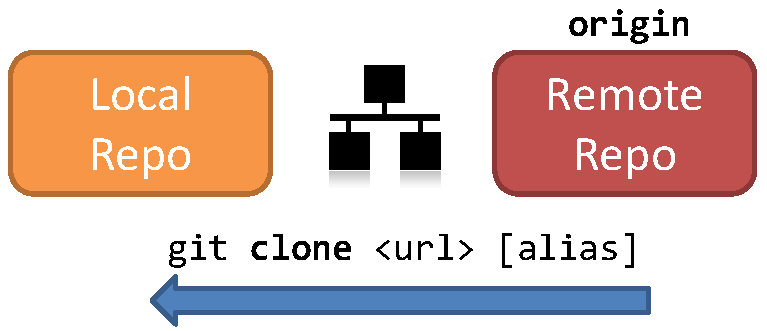
\includegraphics[width=\linewidth]{gitclone-schema.pdf}
  \label{fig:gitclone}
\end{marginfigure}
\marginnote{An optional folder name can be supplied as last argument to rename the top-level directory of the git repository.}
\marginnote{The SSH protocol is implied when using the user@server URL formatting. It is equivalent to ssh://user@server}
We can try to \textbf{clone} an existing Git repository for that.
In the Git jargon, \texttt{clone} consists in copying the entire Git repository from the remote server to the local machine.
As opposed to some centralized SCM tools like SVN, \texttt{git clone} by default will copy every single piece of information necessary to restore all previous versions ever known.
This is why we say Git is distributed: repositories are completely replicated on every machine.

\begin{lstlisting}[style=BashInputStyle]
  $ git clone git@gitlab.server.com:git-training/lesson1 [folder]
\end{lstlisting}

\noindent When the connection is successful, git will clone the repository and give a quite verbose output on what is going on:

\begin{lstlisting}[style=BashInputStyle]
  Cloning into 'lesson1'...
  remote: Counting objects: 23, done.
  remote: Compressing objects: 100% (17/17), done.
  remote: Total 23 (delta 3), reused 0 (delta 0)
  Receiving objects: 100% (23/23), done.
  Resolving deltas: 100% (3/3), done.
\end{lstlisting}

A new folder \texttt{lesson1} should appear in the current directory.
The Git repository (\texttt{.git folder}) and working tree are both contained inside the \texttt{lesson1} directory.
\marginnote{\texttt{lesson1}, like all Git repositories, is self-contained and can be moved around the filesystem without risk.}

\marginnote{The \texttt{.git} folder is the actual repository with all Git objects and settings. We will not go into more details about this in this course, and will ignore it hereafter}
\begin{lstlisting}[style=BashInputStyle]
  $ cd lesson1/
  $ tree -L 2 -a 
  .
  |-- .git
  |   |-- branches
  |   |-- config
  |   |-- description
  |   |-- HEAD
  |   |-- hooks
  |   |-- index
  |   |-- info
  |   |-- logs
  |   |-- objects
  |   |-- packed-refs
  |   `-- refs
  |-- python
  |   `-- calc.py
  `-- README.md
\end{lstlisting}

The \textbf{working tree} is the set of files and folders contained inside the \texttt{lesson1} folder, not including the \texttt{.git}.
\begin{marginfigure}%
  \centering
  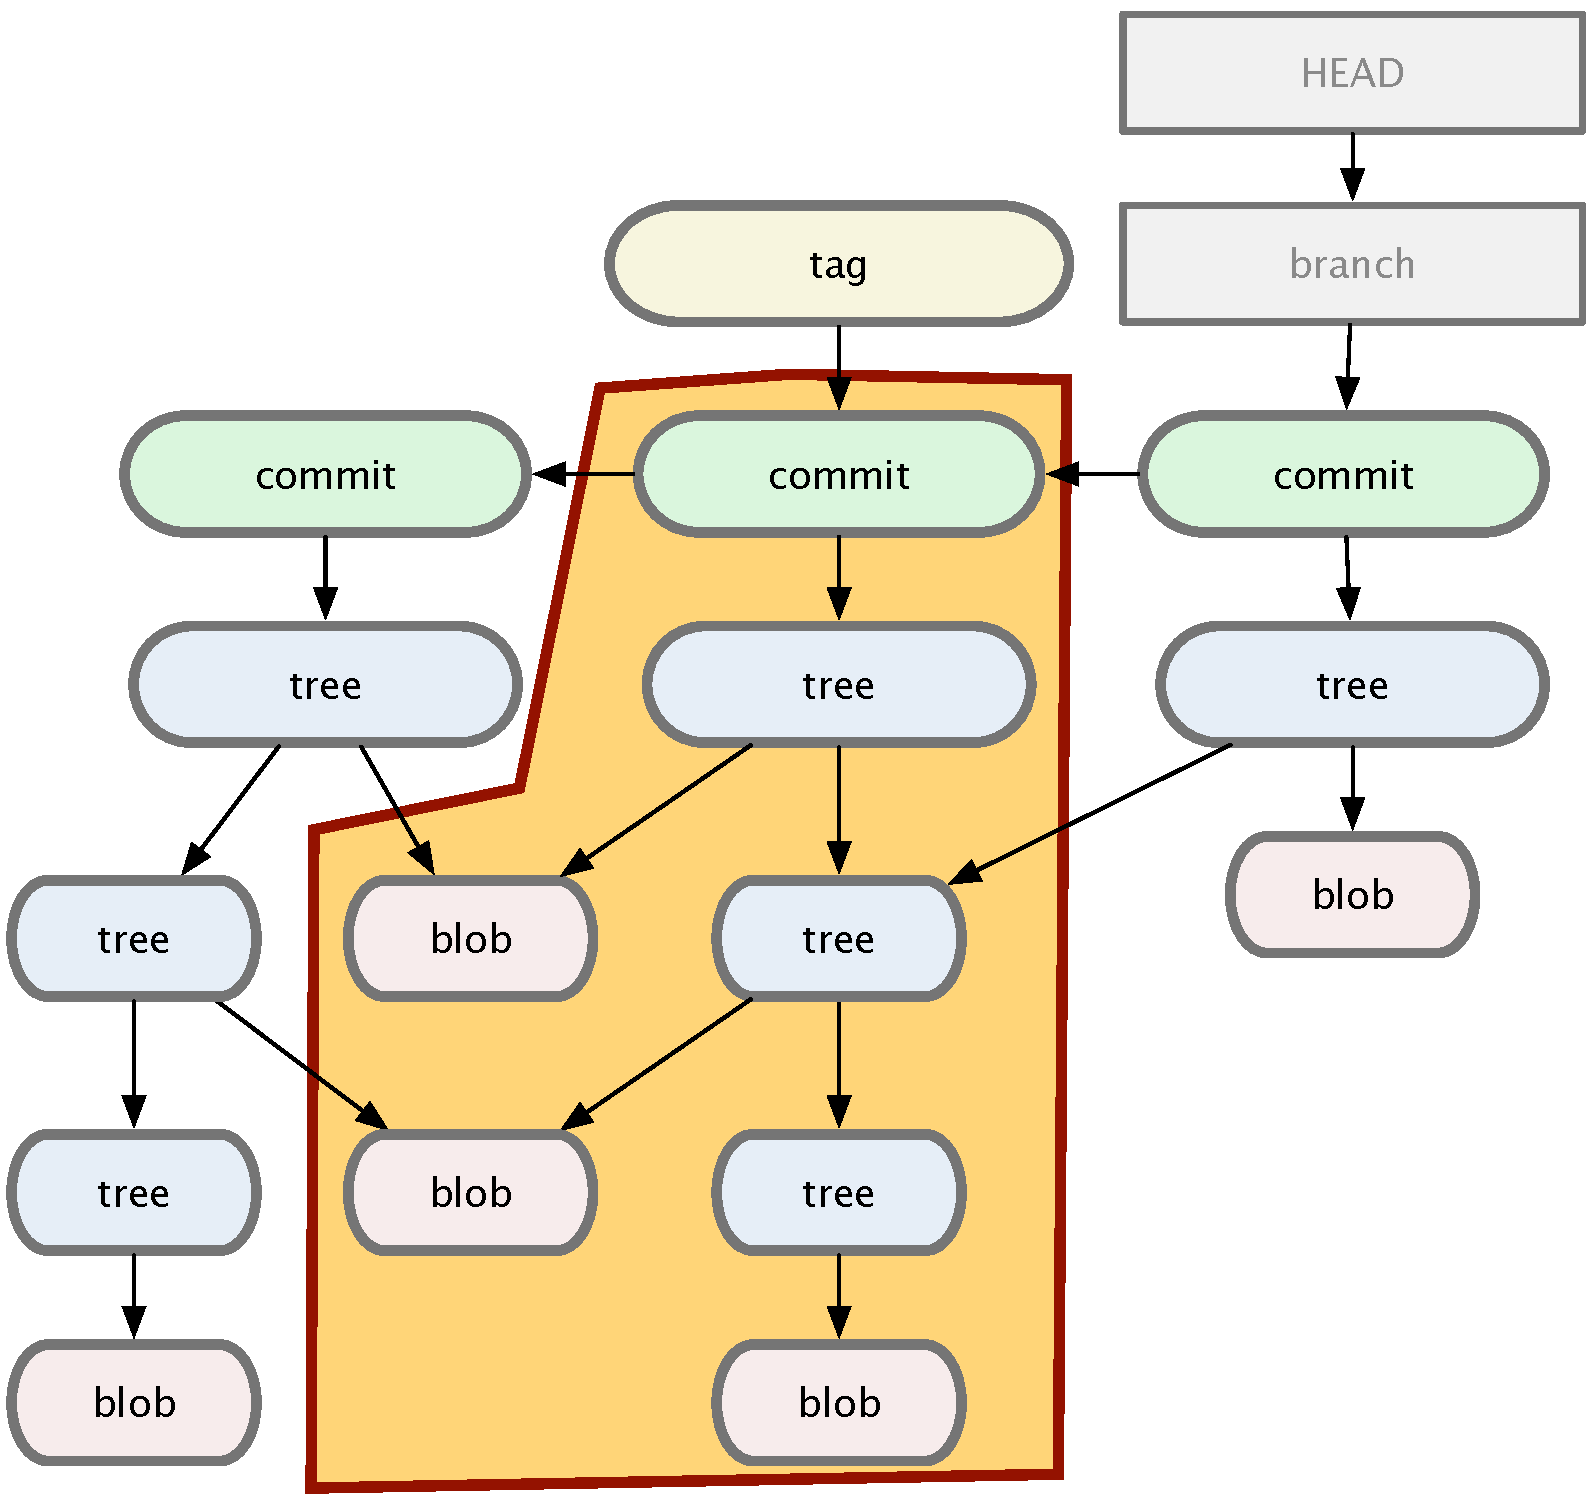
\includegraphics[width=\linewidth]{tree.pdf}
  \label{fig:tree}
  \caption{Representation of an arbitrary working tree for a certain commit. The files checkout out on disk and their folders are represented by blob and tree objects.}
\end{marginfigure}
In our working tree, we have a file called \texttt{README.md} in the root directory, and a \texttt{python} directory containing a single python script.
Only a single \textit{version} of the working tree can be \textit{checked out}, or "on disk" at a given time.

As we have seen in the introductory slides, the working tree is a snapshot of the whole project at a certain point of the history.
A version is uniquely identified by a \textbf{commit} object, containing author/date information and pointing to a top-level \textbf{tree} object and one or more \textbf{parent commits}.
In turn, each \textbf{tree} object contains other \textbf{tree} objects and \textbf{blob} objects, or files.
This course does not cover internal of Git, but you can find more information on Git Objects in the introductory presentation.

\section{Exploring the Repository}

So we have just cloned out first repository, and have seen the difference between the \textbf{working tree} and \textbf{local repository}.
Most of the git commands we use will interact with the local git repository to write and read information to and from the working tree.
Before we actually change anything, let's take a look at the commands available to browse the current status of a project and its history.

\subsection{Listing Remotes}

The \texttt{git clone} command initiated a local repository replicating a \textbf{remote} repository, identified by a URL.
Information related to the state of \textbf{remote} repostories is stored in a dedicated area within the Git repository.
For a name-only list of remotes, we use:

\begin{lstlisting}[style=BashInputStyle]
  $ git remote
  origin
\end{lstlisting}

Every remote is identified by a short-hand name: \textbf{origin} in this case which is the default name Git assigns to a remote when it is cloned.
We can rename a remote repository to give it a more expressive name.
Let's rename it to \texttt{gitlab}, to remind us that the remote is hosted on our local Gitlab server.

\begin{lstlisting}[style=BashInputStyle]
  $ git remote rename origin gitlab
\end{lstlisting}


There is a verbose version of \texttt{git remote} which lists the URLs to each remote.
\marginnote{There are actually 2 URLs defined for each remote, allowing to decouple \texttt{fetch} from \texttt{push} to use different protocols or even different paths for some very specific configurations.}

\begin{lstlisting}[style=BashInputStyle]
  $ git remote -v
  gitlab	git@gitlab.server.com:git-training/lesson1 (fetch)
  gitlab	git@gitlab.server.com:git-training/lesson1 (push)
\end{lstlisting}

We will get back to remotes later, let's just mention that it is possible to add and delete a remote, as well as set a new URL for an existing remote.
For example, we can set an altenate but equivalent notation of the URL:

\marginnote{This is a 1-line command displayed in 2 lines for readability. I use the "\textbackslash" character and an indented second line to represent this.}

\begin{lstlisting}[style=BashInputStyle]
  $ git remote set-url gitlab \
     ssh://git@gitlab.server.com:git-training/lesson1.git
\end{lstlisting}

\subsection{Local and Remote branches}

As we will see throughout this course, \textbf{branches} are omnipresent in Git.
Therefore, commands which list branches and show their relationships are particularly useful.
The simplest way to list branches is:

\marginnote{Omitting the \texttt{-a} option of \texttt{git branch} will display only the local branches.}

\begin{lstlisting}[style=BashInputStyle]
  $ git branch -a
  * `master`
  §remotes/origin/HEAD -> origin/master§
  §remotes/origin/master§
\end{lstlisting}

The output lists local and remote branches.
The local branches are first displayed in default color, with the exeption of the \textbf{currently checked-out} branch, which is displayed in green and has an asterisk next to it.
Here, the current branch is master.

The remote branches are displayed in red and are prefixed with \texttt{remotes/alias/} for readability.
There's a special \texttt{HEAD} pointing on a remote branch which simply identifies the remote branch set as the project's default branch, which will be checked out locally when doing a \texttt{git clone}.

\subsection{Viewing the history}

To view the history of the current branch:

\begin{lstlisting}[style=BashInputStyle]
  $ git log
\end{lstlisting}

This will display a verbose output of the log in a scrollable text viewer.
\marginnote{The log manpage \texttt{git log --help} is a great reference as well as online resources such as \url{http://gitready.com/advanced/2009/01/20/bend-logs-to-your-will.html}
\\ \vspace{0.5cm}
\noindent The last command shows a textual graph of the history. A useful and complete git log graph is given at \url{http://stackoverflow.com/questions/1057564/pretty-git-branch-graphs}}
Git log has plenty of useful options, I will list a few of them here and let you experiment with them.

\begin{lstlisting}[style=BashInputStyle]
  $ git log -n 3
  $ git log --pretty=oneline
  $ git log --pretty=[short, medium, full, fuller, raw...]
  $ git log --pretty=format:'%h - %d %s (%cr) <%an>'
  $ git log --pretty=format:'%h -%C(red)%d%C(reset) %s (%cr) <%an>'
  $ git log --oneline
  $ git log --since "3 hours ago"
  $ git log --since "1 week ago"
  $ git log --graph --pretty=format:' ... '
\end{lstlisting}

\subsection{Graphical overview of branches}

We have seen that there are command-line ways of comparing commits in branches with textual graphs, but this can get complicated when dealing with multiple branches and remotes.
An alternative is to use a graphical user interface, such as Gitk which is distributed in msysgit and included in Linux and MacOS X installations.
To open Gitk:

\begin{marginfigure}%
  \centering
  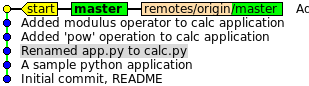
\includegraphics[width=\linewidth]{gitk-start.png}
  \label{fig:gitk-start}
  \caption{Our very simple project displayed in Gitk. There is only 1 local branch with a linear history.}
\end{marginfigure}

\begin{lstlisting}[style=BashInputStyle]
  $ gitk --all
\end{lstlisting}

This is by far the fastest and easiest way to get an overview of the local and remote branches.
In Gitk, the local branches are green, the current local branch is green and bold, and remote branches are prefixed with a peach path.
Our project also has a yellow label, which is a tag.
Like a branch, a \texttt{tag} is little more than a label on a certain commit, the main difference being that a tag is designed to be permanent to label an important point in the project history for future reference (code release, development milestone...), whereas a branch is meant to evolve.
We'll get back to branches and tags later.

\subsection{Working tree status}

We are about to start applying changes to our project.
A useful command to track the status of the different files in Git is \texttt{git status}:

\begin{lstlisting}[style=BashInputStyle]
  $ git status
\end{lstlisting}

As we have not yet modified anything, our git status output is very short:

\begin{lstlisting}[style=BashInputStyle]
  On branch master
  nothing to commit (working directory clean)
\end{lstlisting}

Git status is more verbose when you start changing things.
It will group files in categories according to their state: \textbf{staged}, \textbf{modified} and \textbf{untracked}.

\section{Applying our first changes to master}
In many workflows, it is usually not recommended to work directly on the master branch.
We will do so only this first time to keep things simple.
In the future, we will always apply modifications in isolated branches, and bring these changes back onto master if desireable.

\subsection{Git add to stage an untracked file}

Let's create a new file and see the output of git status:

\begin{lstlisting}[style=BashInputStyle]
  $ echo hello > newfile.txt
  $ git status
  # On branch master
  # Untracked files:
  #   (use "git add <file>..." to include in what will be committed)
  #
    §newfile.txt§
  nothing added to commit but untracked files present (use "git add" to track)
\end{lstlisting}

Git status is more verbose, it tells us that there's untracked content inside the working tree.
All files added to a git working tree are untracked, and will stay untracked unless explicitly defined as tracked content in the repository.

\begin{marginfigure}%
  \centering
  
\includegraphics[width=\linewidth]{gitadd-schema.pdf}
  \label{fig:gitadd}
  \caption{Git add on a file will stage all modifications in the file. It also adds untracked files to the staging area.}
\end{marginfigure}

\begin{lstlisting}[style=BashInputStyle]
  $ git add newfile.txt
  $ git status
    On branch master
    Changes to be committed:
      (use "git reset HEAD <file>..." to unstage)
  
	  `new file:   newfile.txt`
\end{lstlisting}

\subsection{Our first commit}

The staging area is unique to Git, and makes it very powerful.
\marginnote{The term commit is also used in SVN, but it is very different here. An SVN commit is non-reversible and applies changes on the remote repository. A Git commit is a local operation and can easily be undone and edited before it reaches a remote server.}
Successive modifications can be applied until the developer is satisfied with the changes, and is ready to commit them.
Committing changes will define a new point in the project history with a description, and move the HEAD and current branch to the new commit.

\begin{marginfigure}%
  \centering
  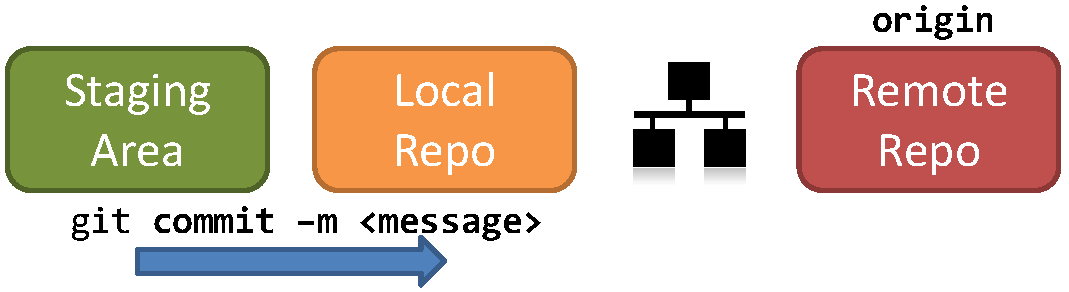
\includegraphics[width=\linewidth]{gitcommit-schema.pdf}
  \label{fig:gitcommit}
  \caption{Git commit creates a new point in history, applying the changes in the staging area.}
\end{marginfigure}

\begin{lstlisting}[style=BashInputStyle]
$ git commit -m "Added new file"
[master 494822d] Added new file
 1 file changed, 1 insertion(+)
 create mode 100644 newfile.txt
\end{lstlisting}

Above, the commit message is given inline with the \texttt{-m} option, but it may be entered via the default text editor by omitting this option.

\subsection{Git add to stage modifications in tracked files}

\section{Applying our changes to a feature branch first}

\begin{lstlisting}[style=BashInputStyle]

\end{lstlisting}

\section{Untracking and Deleting files}

Deleting a file is treated in the same way as other modifications in Git.
The cleanest way to remove a file from disk as well as from the Git repository is to use \texttt{git rm} on it:

\begin{lstlisting}[style=BashInputStyle]
  $ git rm <file>
\end{lstlisting}

This performs two things: it deletes the file from disk, and \textbf{stages} the removal of this file.
The next commit will thus include the deletion of the file.

If you want to untrack a file from Git without deleting it locally, use the \texttt{cached} option:

\begin{lstlisting}[style=BashInputStyle]
  $ git rm --cached <file>
\end{lstlisting}

Git will stage the file to be removed in the next commit, but will not touch the file locally.

\section{}


\bibliography{tufte-latex/sample-handout}
\bibliographystyle{plainnat}



\end{document}
